\chapter{System dynamics and infer-ability}
\ifpdf
    \graphicspath{{Chapter3/Chapter3Figs/PNG/}{Chapter3/Chapter3Figs/PDF/}{Chapter3/Chapter3Figs/}}
\else
    \graphicspath{{Chapter3/Chapter3Figs/EPS/}{Chapter3/Chapter3Figs/}}
\fi

In this section we take a more theoretical approach to parameter estimation and investigate how the global dynamics of the system affect the parameter inference process. The qualitative structure of the solutions of dynamic systems can change as their parameter are varied. These qualitative changes in the dynamics are called bifurcations and the parameter values at which they happen are called bifurcation points. There are different kinds of bifurcations depending on different changes in the dynamics of the system. Here we are concerned with bifurcations that give rise to limit cycles in the phase plane of the solutions and therefore are capable of producing oscillatory behaviour.  Oscillators are present in many biological systems: cell cycles, circadian rhythms, calcium oscillations, pace maker cells, protein responses. Their behaviour in theoretical models is often captured through limit cycle oscillators which are driven by different kinds of bifurcations. In this section we will investigate two bifurcation capable of creating/destroying limit cycles in two-dimensional systems, Hopf Bifurcation and Saddle-Node bifurcation of Invariant Cycle(SNIC). Systems driven by these bifurcations have been used for real and synthetic oscillatory systems in biology. Their dynamics have also been contrasted in designs of the same synthetic genetic oscillator logical motif \cite[] {guantes2006dynamical}.  Since models that use these kinds of bifurcations are used extensively in biology, it is of value to investigate the challenges associated with parameter estimation in those types of models.

In Hopf Bifurcation as the control parameter passes through the bifurcation point, a fixed point of the system loses its stability and the systems shows a limit cycle around that fixed point. In general before the bifurcation point, when the system is temporally perturbed we have damped oscillations which decay and settle down to an equilibrium state(stable fixed point). However in the presence of noise the perturbations are constant and the system does not settle down and therefore it been shown that sustained oscillations can be produced albeit with fluctuating amplitude. After the value of the control parameter passes through the bifurcation point the fixed point loses its stability, a limit cycle is formed around the fixed point and the systems shows sustained oscillations.  Both mechanisms, limit-cycle oscillator with unstable fixed point and noise-induced oscillator with stable fixed point, have been proposed as a driving force for oscillatory systems.

In SNIC bifurcation a limit cycle appears as  fixed points are created from nothing when the control parameter passes through the bifurcation point. In this case however the stability of the fixed point does not change.

\section{Methods}
\subsection{Models}
For our investigation of the effects of a Hopf bifurcation we chose a very simple system that undergoes a Hopf bifurcation\cite[p.250] {strogatz2001nonlinear}. The simplicity of the model is convenient for our investigation while still maintaining the relevant characteristics. The system given in polar coordinates,
\begin{equation}
\begin{array}{lcl}
\dot r &= & \mu r -r^3 \\
\dot \theta &= & \omega + b r^2.
\end{array}
\end{equation}
The system has three parameters: $\mu, \omega, b$. The control parameter for the bifurcation is $\mu$ so we consider the other two known, $(\omega, b)=(1,1)$ and investigate the behaviour as $\mu$ varies. The system has a fixed point $(0,0)$ which undergoes a Hopf Bifurcation losing its stability as the control parameter $\mu$ goes through $0$.

For our investigation of the effects of the SNIC bifurcation we again chose a very simple system\cite[p.250] {strogatz2001nonlinear}. The system in polar coordinates,
\begin{equation}
\begin{array}{lcl}
\dot r &= & \mu r +r^3 - r^5 \\
\dot \theta &= & \omega + b r^2.
\end{array}
\end{equation}
The control parameter for the bifurcation is $\mu$. The radial equation $\dot r =  \mu r +r^3 - r^5$ undergoes a saddle-node bifurcation of fixed points at $\mu=-1/4$ and two new fixed points are created. When view in the two-dimensional setting these correspond to the creation of limit cycles.
\subsection{Maximum Likelihood for ODEs}
\label{sec:likelihood}
For any mathematical model our goal is to infer true parameters $\theta^*$ given some observed data $\mathbf{Y_{d}} =\{\mathbf{y_{t_1}}, \mathbf{y_{t_2}}, \dots, \mathbf{y_{t_M}}\}$ at times $\{t_{i}\}_{1 \le i \le M}$. To this end we wish to know the likelihood function $L(\theta | \mathbf{Y_{d}})$ which tells us how the probability of observing the data $\mathbf{Y_{d}}$ changes with $\theta$. However, a direct approach to obtaining the likelihood function is not possible for deterministic system of ODEs but subject to some assumptions the likelihood function is equivalent to the distance or error between real(observed) and predicted data. That means that the probability of observing the data $\mathbf{Y_{d}}$ for parameter vector $\theta_{s}$ is equivalent to $\Delta(\mathbf{Y_{d}}, \mathbf{Y_{\theta_s}})$ where $\mathbf{Y_{d}}$ is the real data,$\mathbf{Y_{d}}$ data simulated with parameter $\theta_{s}$ and $\Delta$ is the Euclidean distance. This is also the intuition behind using comparisons of real and simulated data with the Euclidean distance as an approximation for the Likelihood function in the ABC algorithms. 

Here we follow the likelihood approach for ODE parameter estimation given in \cite{}. We assume that any observed data point $\mathbf{y_{t_i}}$ is distributed according to $\mathcal{N}(\boldsymbol{\mu}_{t_i}(\theta), \Sigma_{t_i})$, where $\boldsymbol{\mu}_{t_i}(\theta)$ is the solution of the system $\dot x = \mathbf{F}(\mathbf{x}, t, \theta)$ at time $t_i$ and $\Sigma_i$ is a covariance matrix which is the same for all $i$. Then the likelihood function is given by:
\begin{equation}
L(\theta | \mathbf{Y_d}) = \prod_{i=1}^M \frac{1}{(2\pi)^{3/2}|\Sigma|^{1/2}} \exp \left(-\frac{1}{2}(\mathbf{y_{t_i}} - \mu_i(\theta))^{T}\Sigma^{-1}(\mathbf{y_{t_i}} - \mu_i(\theta)) \right).
\end{equation}
We will investigate the behaviour through the log-likelihood function,
\begin{equation}
\begin{array}{lcl}
ln(L(\theta|\mathbf{Y_d}) &= & M ln\left(\frac{1}{(2\pi)^{3/2}|\Sigma|^{1/2}}\right) -\frac{1}{2}\sum_{i=1}^{M}((\mathbf{y_{t_i}} - \mu_i(\theta))^{T}\Sigma^{-1}(\mathbf{y_{t_i}} - \mu_i(\theta))\\
& \propto & -\frac{1}{2}\sum_{i=1}^{M}(d_{\Sigma}(\mathbf{y_i} - \boldsymbol{\mu_i(\theta)}))^2,
\end{array}
\end{equation}
where $d_{\Sigma}(\mathbf{y_i} - \boldsymbol{\mu_i(\theta)}) = \sqrt{(\mathbf{y_{t_i}} - \mu_i(\theta))^{T}\Sigma^{-1}(\mathbf{y_{t_i}} - \mu_i(\theta)}$ is the Mahalanobis distance between $\mathbf{y_{t_i}}$ and $\boldsymbol{\mu_i(\theta)}$ with respect to $\Sigma$.  Subject to our assumption that the covariance matrix $\Sigma$ is equal for $i$ then the Mahalanobis distance is equivalent to Euclidean distance and the log-likelihood function is given by,
\begin{equation}
ln(L(\theta|\mathbf{Y_d}) = -\frac{1}{2}\sum_{i=1}^{M}(d(\mathbf{y_{t_i}}, \mu_{i}(\theta)))^2,
\end{equation}
where $d(\mathbf{y_{t_i}}, \mu_{i}(\theta))$ is the Euclidean distance between $\mathbf{y_{t_i}}$ and$\mu_{i}(\theta))$. It is clear that maximising the 
likelihood function is equivalent to minimising the distance function $d$. Obviously the maximum likelihood estimate will be at the value of the true parameter where real and simulated data are the same and the distance value is equal to $0$. Therefore this likelihood function is related to the problem of finding how far apart are solutions with the same initial conditions as the parameters vary. This is how the likelihood function is also related to the parameter inference process. The landscape of the likelihood function around the true parameter value can give some information on how easy the parameter estimation process will be. For example flat regions imply regions of highly likely values which are close to the true solution therefore suggesting high acceptance rates in the filtering process of ABC schemes. In the next section we investigate how the shape of the likelihood function and consequently the parameter estimation process changes as the systems undergo a bifurcation.

\section{Results}
%Hopf bifurcation=============================
\subsection{Hopf Bifurcation}
\begin{table}[ht]
\centering
\begin{tabular}{cc}
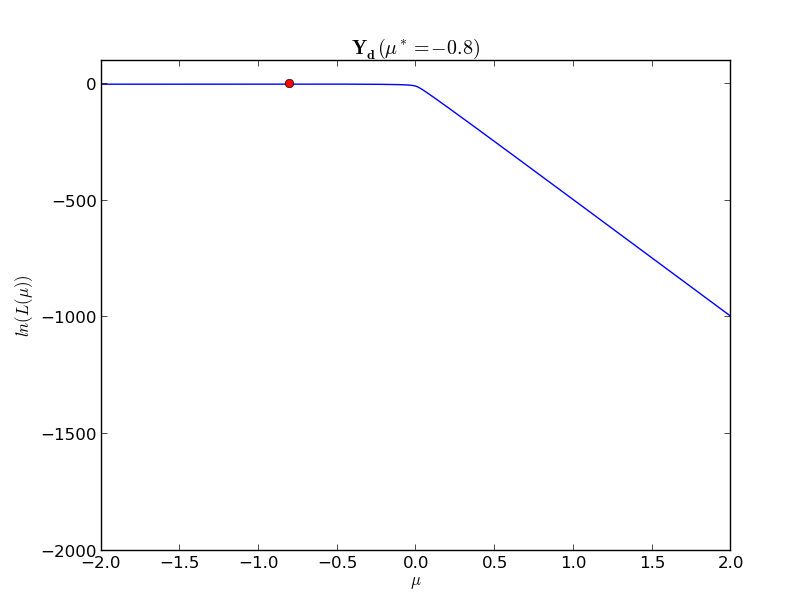
\includegraphics[scale=0.3]{likelihood_hopf08m}&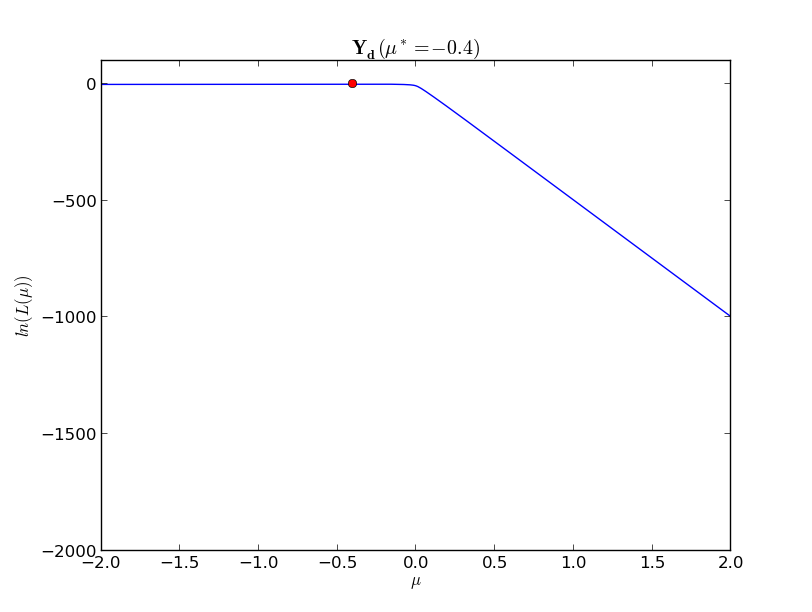
\includegraphics[scale=0.3]{likelihood_hopf04m}\\
\newline
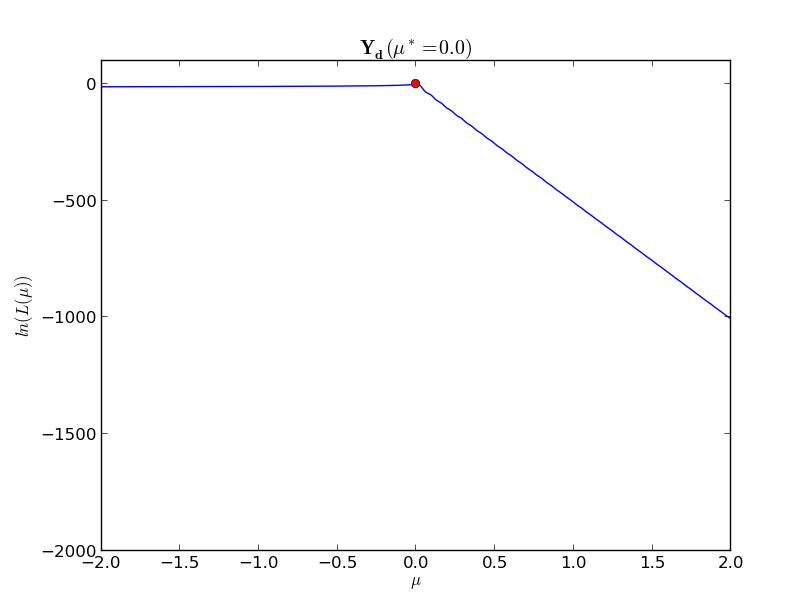
\includegraphics[scale=0.3]{likelihood_hopf0}&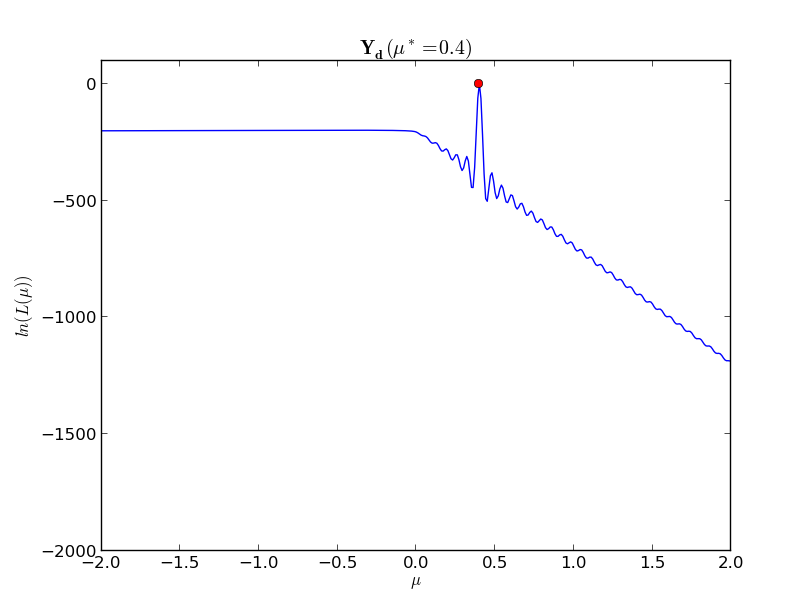
\includegraphics[scale=0.3]{likelihood_hopf04}\\
\newline
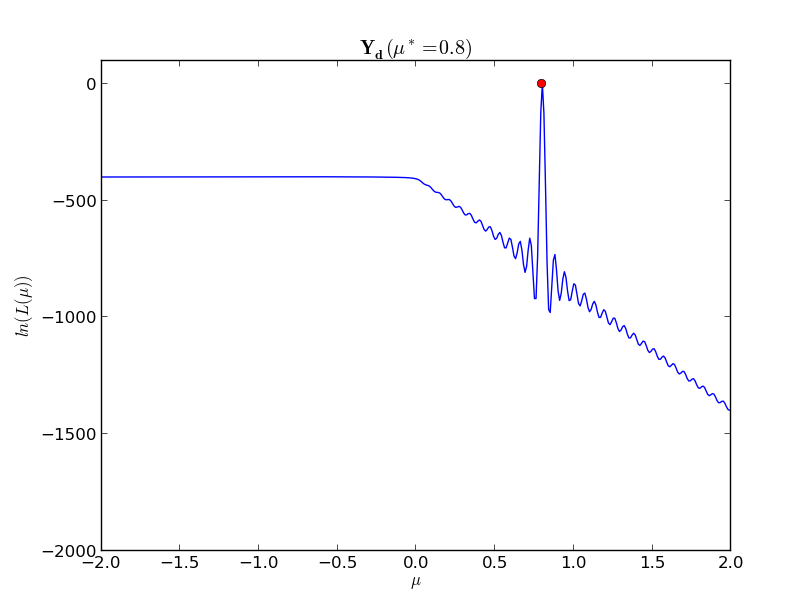
\includegraphics[scale=0.3]{likelihood_hopf08}&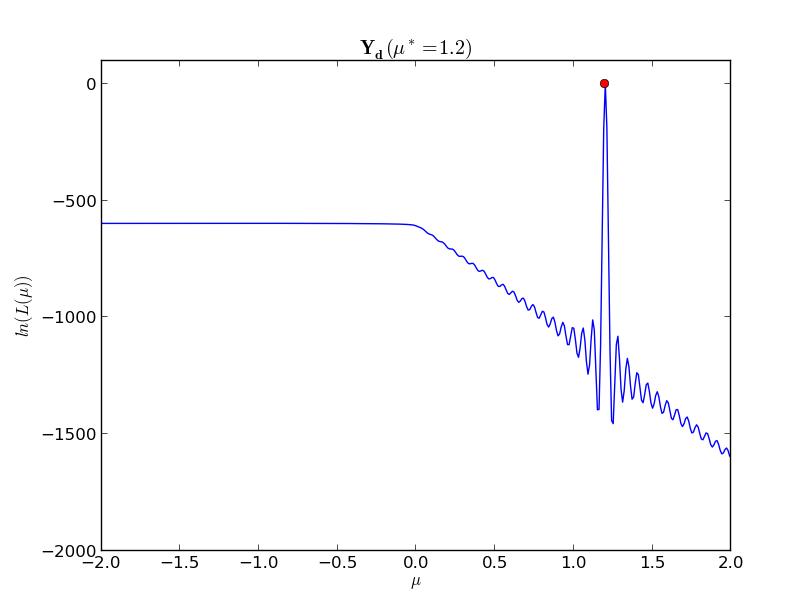
\includegraphics[scale=0.3]{likelihood_hopf12}\\
\end{tabular}
\caption{Log-likelihood plots for different values of $\mu^*$ specified in the header. The maximum likelihood is denoted by the red dot which is as expected at the true value.}
\label{fig:hopf}
\end{table}
To understand the effects of Hopf bifurcation we plot the log-likelihood function, $\text{ln}(L(\mu | \mathbf{Y_{d}}(\mu^*)))$ for parameter $\mu$ which is the control parameter for the bifurcation, for different values of $\mu^*$ both sides of the bifurcation point. The resulting plots are in \ref{fig:hopf}. As expected the maximum likelihood estimator is at the true value. However there is a big qualitative change in the shape of the log-likelihood functions when $\mu > 0$ and when $\mu < 0$. 

For the landscape of the log-likelihood plot for values $\mu^* < 0$ we observe a relatively flat region in the interval [-2.0, 0.0] and then a relatively steep part with negative gradient in the interval [0.0, 2.0]. The flat part in the region $-2 \le \mu \le 0$ tells us that parameter estimates in that domain are all highly likely.This is easy to understand as the corresponding solutions for estimates in that domain  are qualitatively similar to each other and to the solution for $\mu^*$. Therefore the distance between them and also between them and the solution for $\mu^*$ is small which is reflected on the likelihood plot. As the value of $\mu$ goes through the bifurcation point, the estimates become increasingly unlikely which can also be explained by the fact that the solutions corresponding to estimates in this domain are qualitatively very different from the solution for $\mu^*$. Moreover the bifurcation point at $\mu = 0$ which marks the point of change in system dynamics also marks the change in the behaviour and shape of the likelihood function.

For the landscape of the log-likelihood plot at the other side of the bifurcation for values $\mu^* > 0$ we observe the maximum likelihood estimate, as expected at the true value, but this occurs at a spike in the curve. That tells us that solutions that correspond to parameter estimates which are near the true value $\mu^*$ are not very likely so small changes in the control parameter near the true value $\mu^*$ result to big changes in the corresponding solution. Again the bifurcation point at $\mu=0$ is recognisable by the change in the behaviour of the graph at that point. Solutions for estimates in the region [-2, 0] are similar so their distances from the solution for true parameter value are similar, hence the flat part of the graph.On the other hand solutions corresponding to estimates in the region [0, 2] are relatively dissimilar, hence the bigger changes in the distances to the true solution we observe via a steeper descent in the graph in that region.

To understand the change in the distances between adjacent and solutions and the change in the shape of the likelihood function as the control parameter goes through the bifurcation point we can look at what happens to the system dynamics. This will be easier if we look at solutions as trajectories in the phase plane\ref{fig:phase_plane_hopf}. At one side of the bifurcation point for values of $\mu^* < 0$ the fixed point of the system is stable therefore trajectories near the fixed point will get attracted to it. This makes solutions for nearby parameter estimates in that region qualitatively very similar which makes the distance between them very small. Given the equivalence of distance with likelihood, we expect estimates in that region to be highly likely which is verified by our findings. When the control parameter passes through the bifurcation point, the fixed point of the system becomes unstable therefore trajectories that start near it will be pushed away from it towards the limit cycle around it. This makes solutions that start from the same initial conditions more dissimilar and the distance between them higher. In order to approach the observed data for $\mu^*$ the parameter estimate will have to be close to it.
\begin{table}[ht]
\centering
\begin{tabular}{cc}
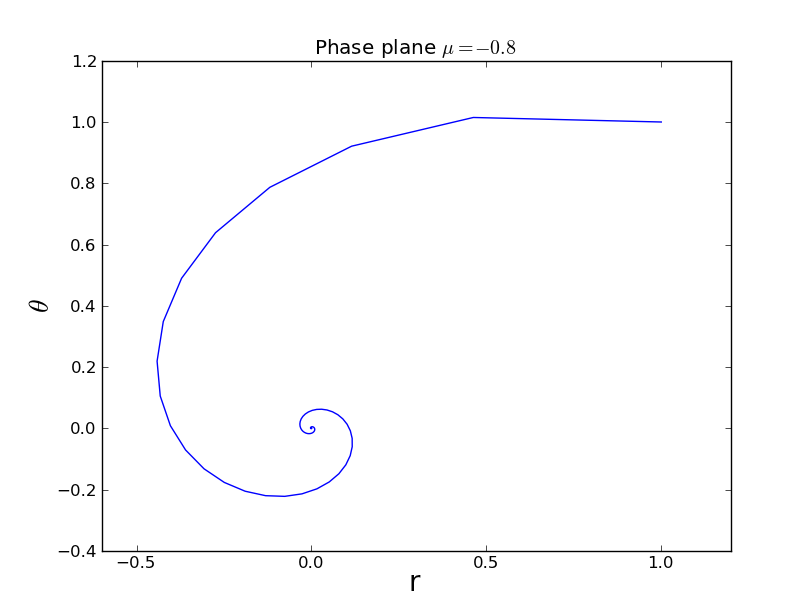
\includegraphics[scale=0.3]{phase_hopf08m}&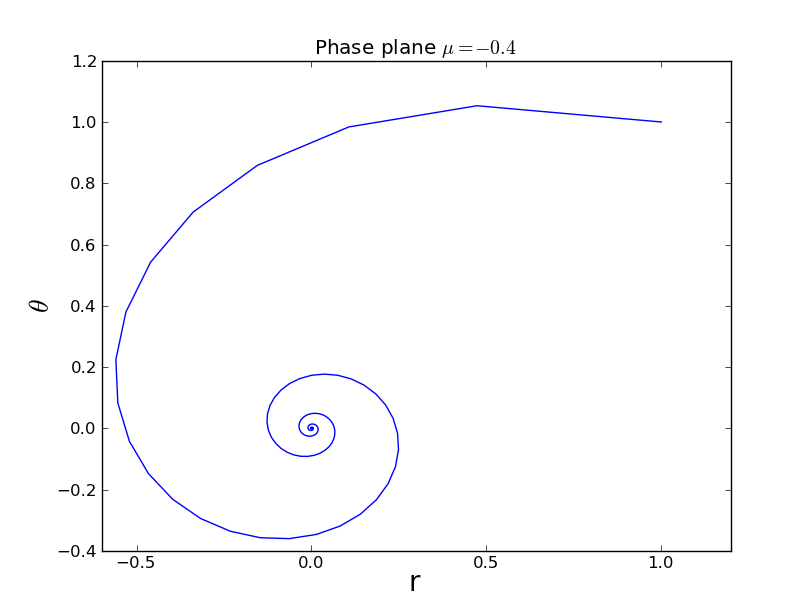
\includegraphics[scale=0.3]{phase_hopf04m}\\
\newline
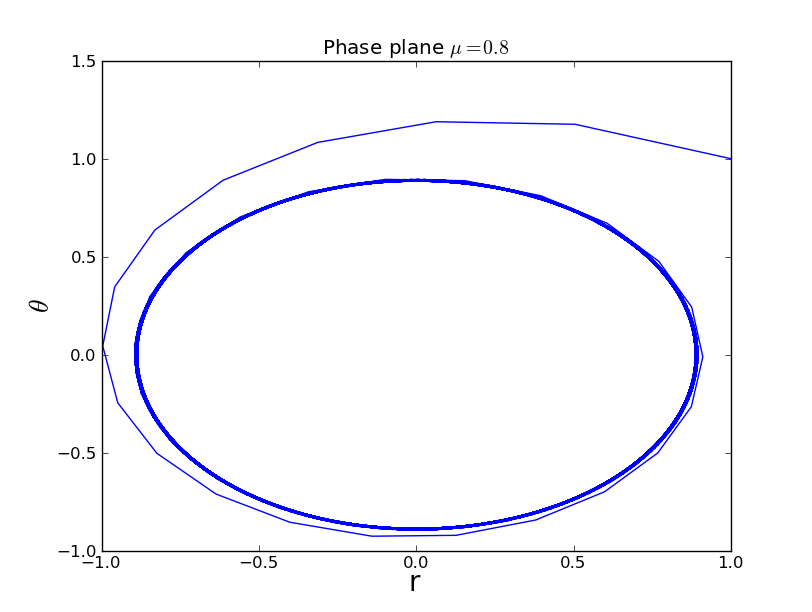
\includegraphics[scale=0.3]{phase_hopf08}&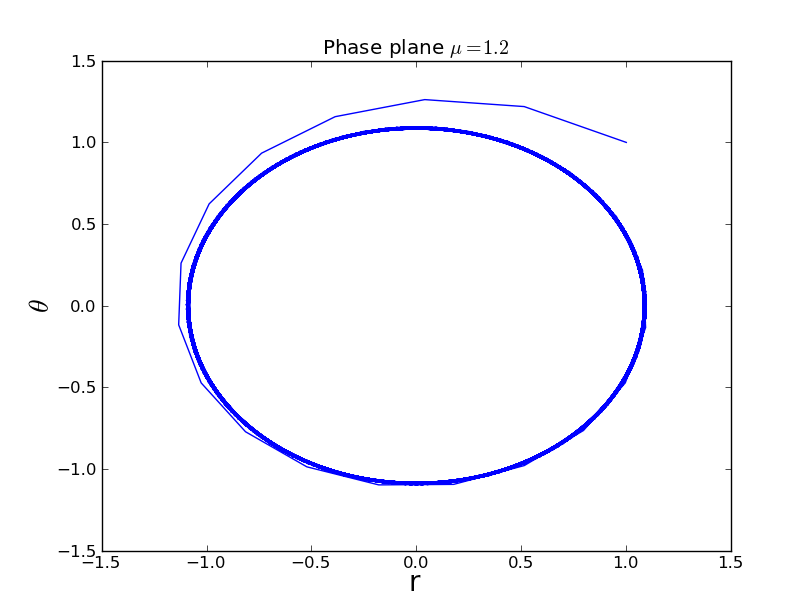
\includegraphics[scale=0.3]{phase_hopf12}\\
\end{tabular}
\caption{Solutions corresponding to trajectories in the phase plane for different value of
control parameter $\mu$ either side of the bifurcation point $\mu = 0$.}
\label{fig:phase_plane_hopf}
\end{table}

The connection between the shape of the likelihood function and the distance between nearby solutions and the practicalities of the parameter inference process should be apparent. For values $\mu^* < 0$ nearby solutions are similar so we expect a high acceptance rate and less iteration steps at the filtering steps of ABC schemes that use the distance function as a filter. The population obtained from the ABC scheme however will be spread out(high variance) which might decrease the confidence for the estimate. On the other hand from the other side of the bifurcation point and for values $\mu^* > 0$ where nearby solutions are not very similar we expect a lower acceptance rate and more iterations steps. But we expect the obtained population to be more concentrated giving a higher confidence for the estimate. These are indeed verified as we test the SMC scheme for%give resutls

There is a also an apparent link between the shape of the likelihood function and parameter sensitivity. A spike in the log-likelihood curve tells us that a the system is very sensitive to changes in that parameter. Small changes in the parameter value get amplified in the solution. On the other hand a relatively flat region around the true parameter value tells us that the model is not very sensitive to that parameter as changes to it result in small changes in the corresponding solutions. Hence this is another way to see the importance of the rich information obtained from ABC schemes. ABC schemes return a distribution for the parameter estimate instead of a single value. As we have seen populations of parameter estimates that are concentrated around a specific value with low variance imply low likelihood estimates around the true parameter. This can be translated to a spike in the shape of the log-likelihood function, for example in \ref{} and therefore to high sensitivity of the system to that parameter. Populations of parameter estimates which are more spread out with high variance imply highly likely estimates around the true parameter value and hence a flat region of the likelihood function which tells us that the system is not very sensitive to that parameter.


\subsection{SNIC}
\begin{table}[ht]
\centering
\begin{tabular}{cc}
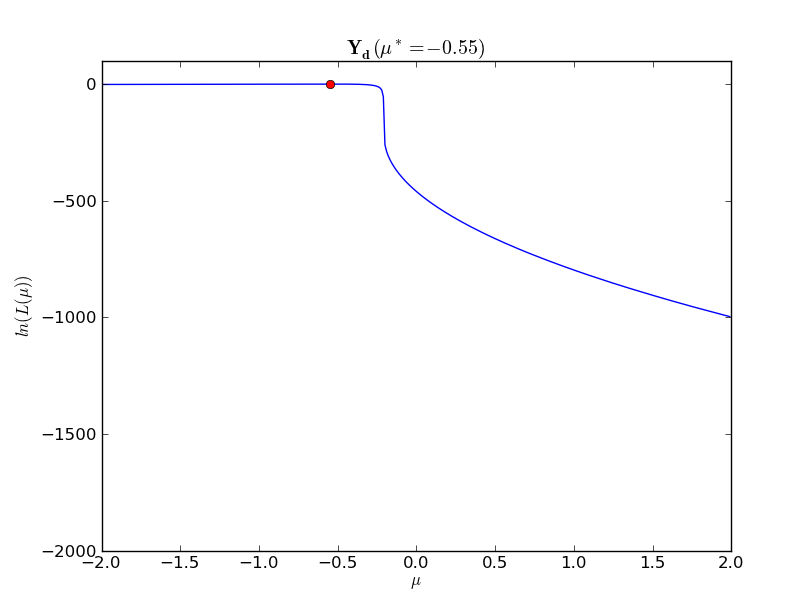
\includegraphics[scale=0.3]{likelihood_sinc_055m}&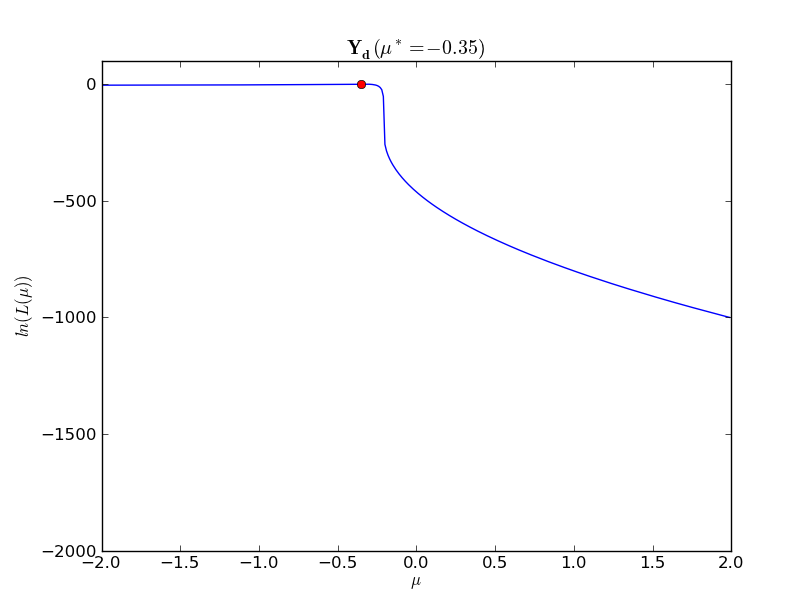
\includegraphics[scale=0.3]{likelihood_snic035m}\\
\newline
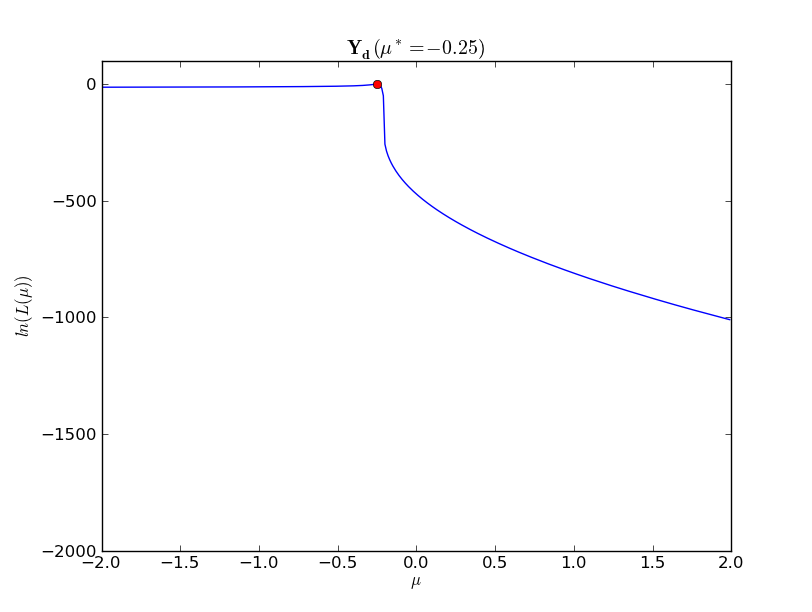
\includegraphics[scale=0.3]{likelihood_snic025m}&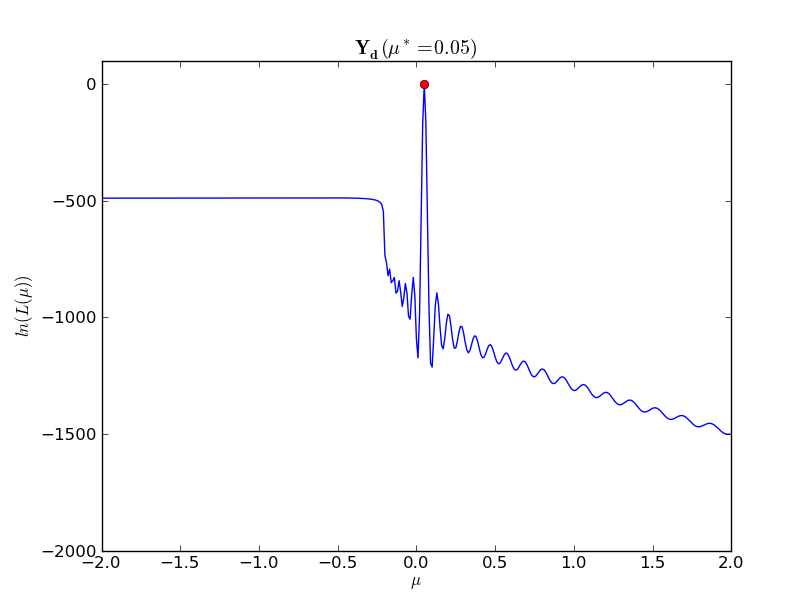
\includegraphics[scale=0.3]{likelihood_snic005}\\
\newline
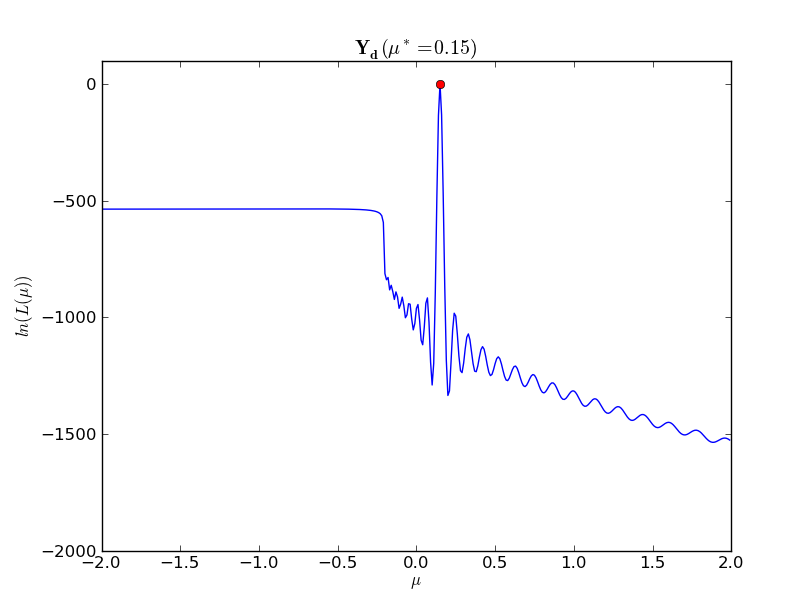
\includegraphics[scale=0.3]{likelihood_snic015}
\end{tabular}
\caption{Log-likelihood plots for different values of $\mu^*$ specified in the header. The maximum likelihood is denoted by the red dot which is as expected at the true value.}
\label{fig:snic}
\end{table}
We proceed to investigate the effects of the SNIC bifurcation in the same way as we have for the the Hopf bifurcation. We plot the likelihood function $\text{ln}(L(\mu | \mathbf{Y_{d}}(\mu^*)))$ for values of $\mu^*$ either side of the bifurcation point at $\mu = -1/4$ for a range of values of $\mu$ in the range [-2, 2] taken at regular intervals of $0.01$. The resulting log-likelihood plot are in Figure\ref{fig:snic}. As expected the maximum likelihood estimator is always at the true value $\mu^*$, however we again notice a qualitative change in the plots either side of the bifurcation point.

For the landscape of the plots of log-likelihood functions for values of parameter before the bifurcation point $\mu^* < -1/4$ there is flat region in the area from [-2, -1/4], then an elbow in the curve at the bifurcation point and then a steeper area with negative gradient. This is qualitatively the same as the log-likelihood functions at one side of the Hopf bifurcation point in the previous section. The flat part tells us that solutions in that range are all relatively close to the true solution and the steep part that solutions in that area become increasingly unlikely. Again this change is due to the change in the system dynamics either side of the bifurcation point.

For the landscape of the plots of log-likelihood function for values of parameter after the bifurcation again we get similar results as in the Hopf bifurcation case when the limit cycle appears in the phase plane. The maximum likelihood estimate at the true value happens as a spike in the curve which tells us that nearby estimates are unlikely so solutions that start at the same initial condition vary considerably as the parameters change. 
\begin{table}[ht]
\centering
\begin{tabular}{cc}
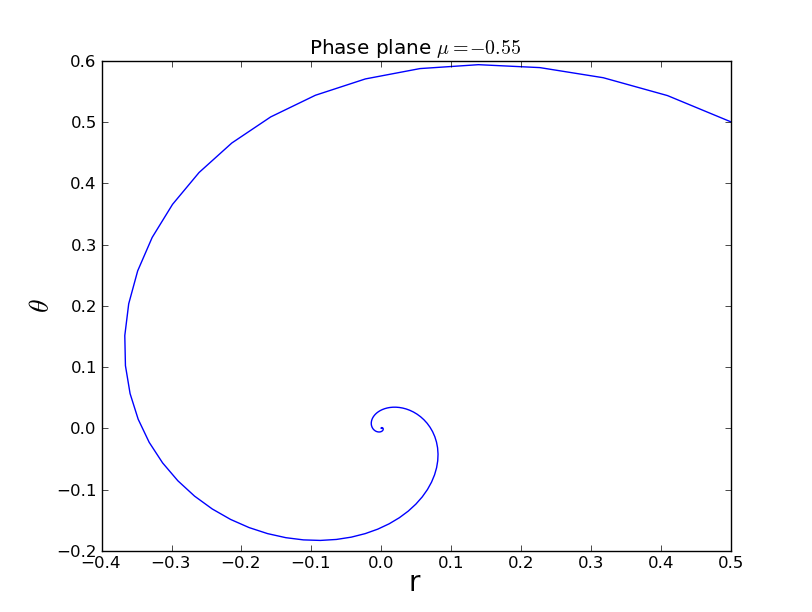
\includegraphics[scale=0.3]{phase_snic055m}&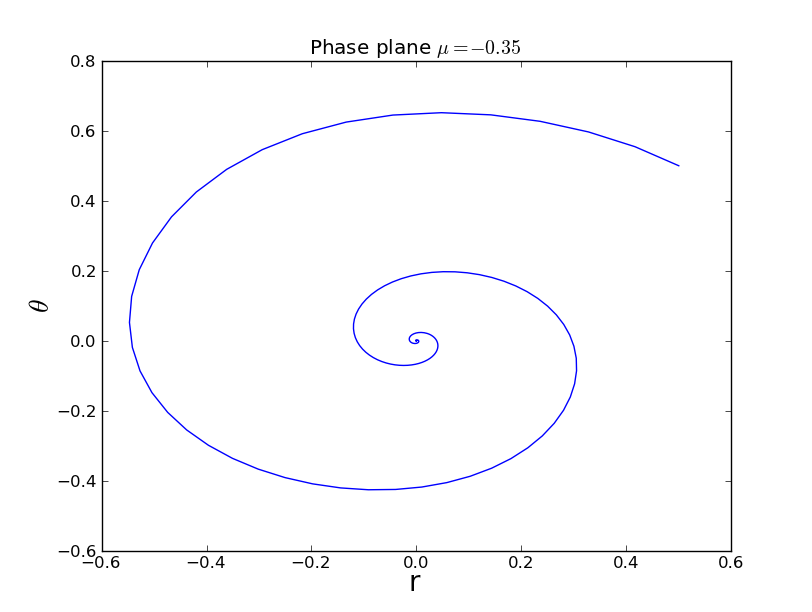
\includegraphics[scale=0.3]{phase_snic035m}\\
\newline
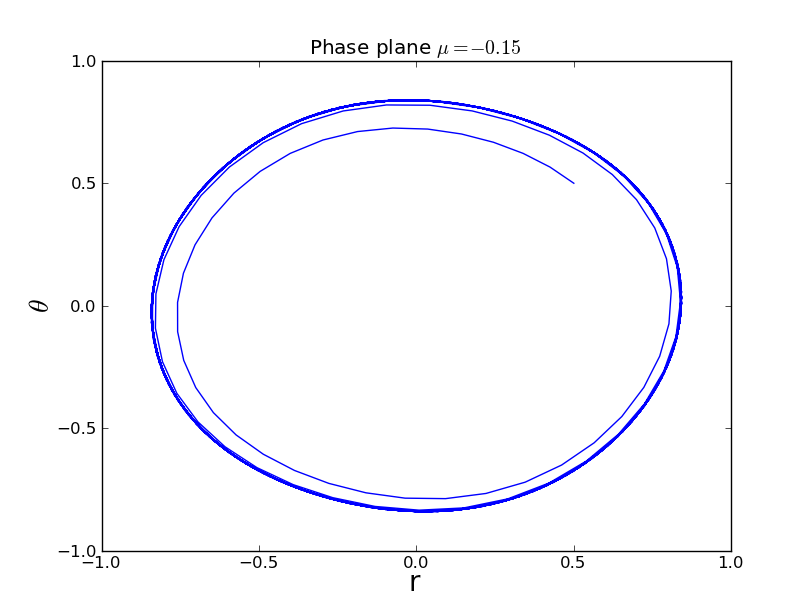
\includegraphics[scale=0.3]{phase_snic015m}&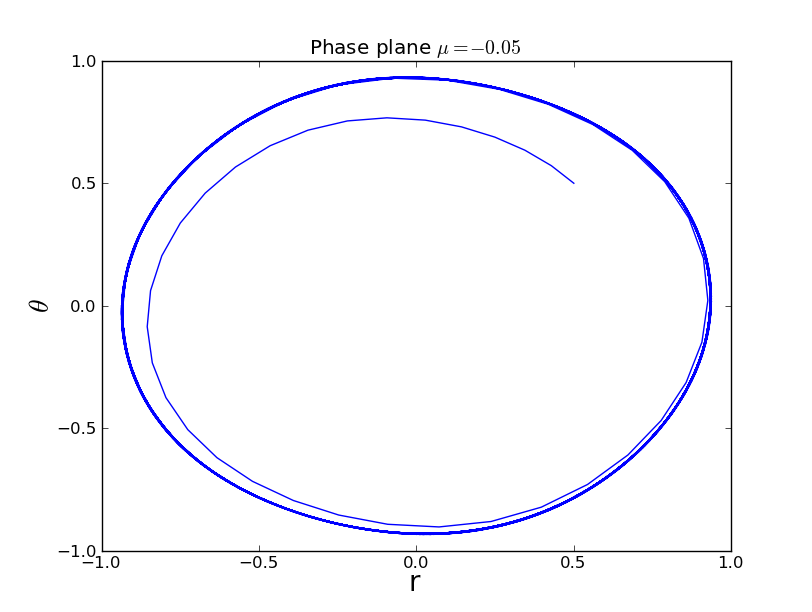
\includegraphics[scale=0.3]{phase_snic005m}\\
\end{tabular}
\caption{Solutions corresponding to trajectories in the phase plane for different value of
control parameter $\mu$ either side of the bifurcation point $\mu = 0$.}
\label{fig:phase_plane_hopf}
\end{table}
The findings can again be explained by the change to the system dynamics as the system undergoes the bifurcation and to the corresponding solutions as trajectories in the phase plane. For values of the control parameter before the bifurcation point $\mu < -1/4$ the fixed points in the radial equation annihilate each other as it undergoes a saddle-node bifurcation and the limit cycles are destroyed. The fixed point is stable though so trajectories starting near it will get drawn towards it. In that way solutions resemble solutions of the Hopf bifurcation system before the bifurcation point. Because solutions get drawn towards the fixed point which makes solution for different parameter values qualitatively very similar hence the flat part in the region. After the control parameter goes through the bifurcation point at $\mu=-1/4$ the fixed point does not lose its stability as in the Hopf bifurcation case but two fixed points appear in the radial equation which correspond to limit cycles in the two-dimensional case. Therefore solutions that start near that fixed point will get pushed out to the limit cycle which is the same kind of behaviour that we get from the Hopf bifurcating system in the previous section. Nearby solutions will be qualitatively not very similar unless their corresponding control parameter values are really close hence the spike in the log-likelihood curves for $\mu > -1/4$.

So we have found that the two bifurcation that can create limit cycles in the two-dimensional case behave similarly as limit cycles are created even though the mechanism for their creation is not the same. 

%
%link the shape of the likelihhod function with parameter estimation process, get practical results...choose a system ...graph the likelihhood function both sites of a bifurcation point etc. etc., do a 2 parameter likelihhood surface plot as well
% ------------------------------------------------------------------------


%%% Local Variables: 
%%% mode: latex
%%% TeX-master: "../thesis"
%%% End: 
